\chapter{Background}
\label{background}

\section{Technologies}

There are a number of components needs to build the architecture of a web application. The nature of these components is explored below, and their contribution to the creation of a web application is analysed.

\subsection{Web Application Framework}
The Web Application Framework [WAF] chosen for this project is Spring MVC. Shan and Hua define a WAF as “a defined support structure in which other software applications can be organized and developed”. (Shan and Hua 2006). MVC, or Model-View-Controller, is a software pattern that facilitates the use of a user interface. The Model manages the behaviour and data of the application. The View will manage the information obtained from the model and display it to the user. The Controller takes user input, such as key strokes, mouse movements or a touch display, and can interact and invoke functionality within the Model and/or View.

Spring MVC has a \textit{DispatcherServlet}, defined within \textit{web.xml} in the WEB-INF folder, which will try to load the application context from a servlet file, defined within this application as \textit{member-servlet.xml}. The \textit{DispatcherServlet} is responsible for handling the initial HTTP request from the browser. Once it receives this request, it consults the HandlerMapper, which calls the appropriate Controller. A HandlerMapper takes a value, such as "/admin", and checks which controller handles this mapping. The Controller will take this request, and call the appropriate method, or methods, and interact with the Service layer of the application, if necessary. The View name is then returned to the \textit{DispatcherServlet}, which in turn passes the value to the ViewResolver. A ViewResolver provides a mapping between a \textit{view name} and the \textit{view}, that is to say, the web page requested. Once this view is finalised, the \textit{DispatcherServlet} passed any model created within the Controller to the View, which is then rendered by the browser. This process is shown in Figure ~\ref{fig:dispatcherflow}


\begin{table}[H]
\begin{center}
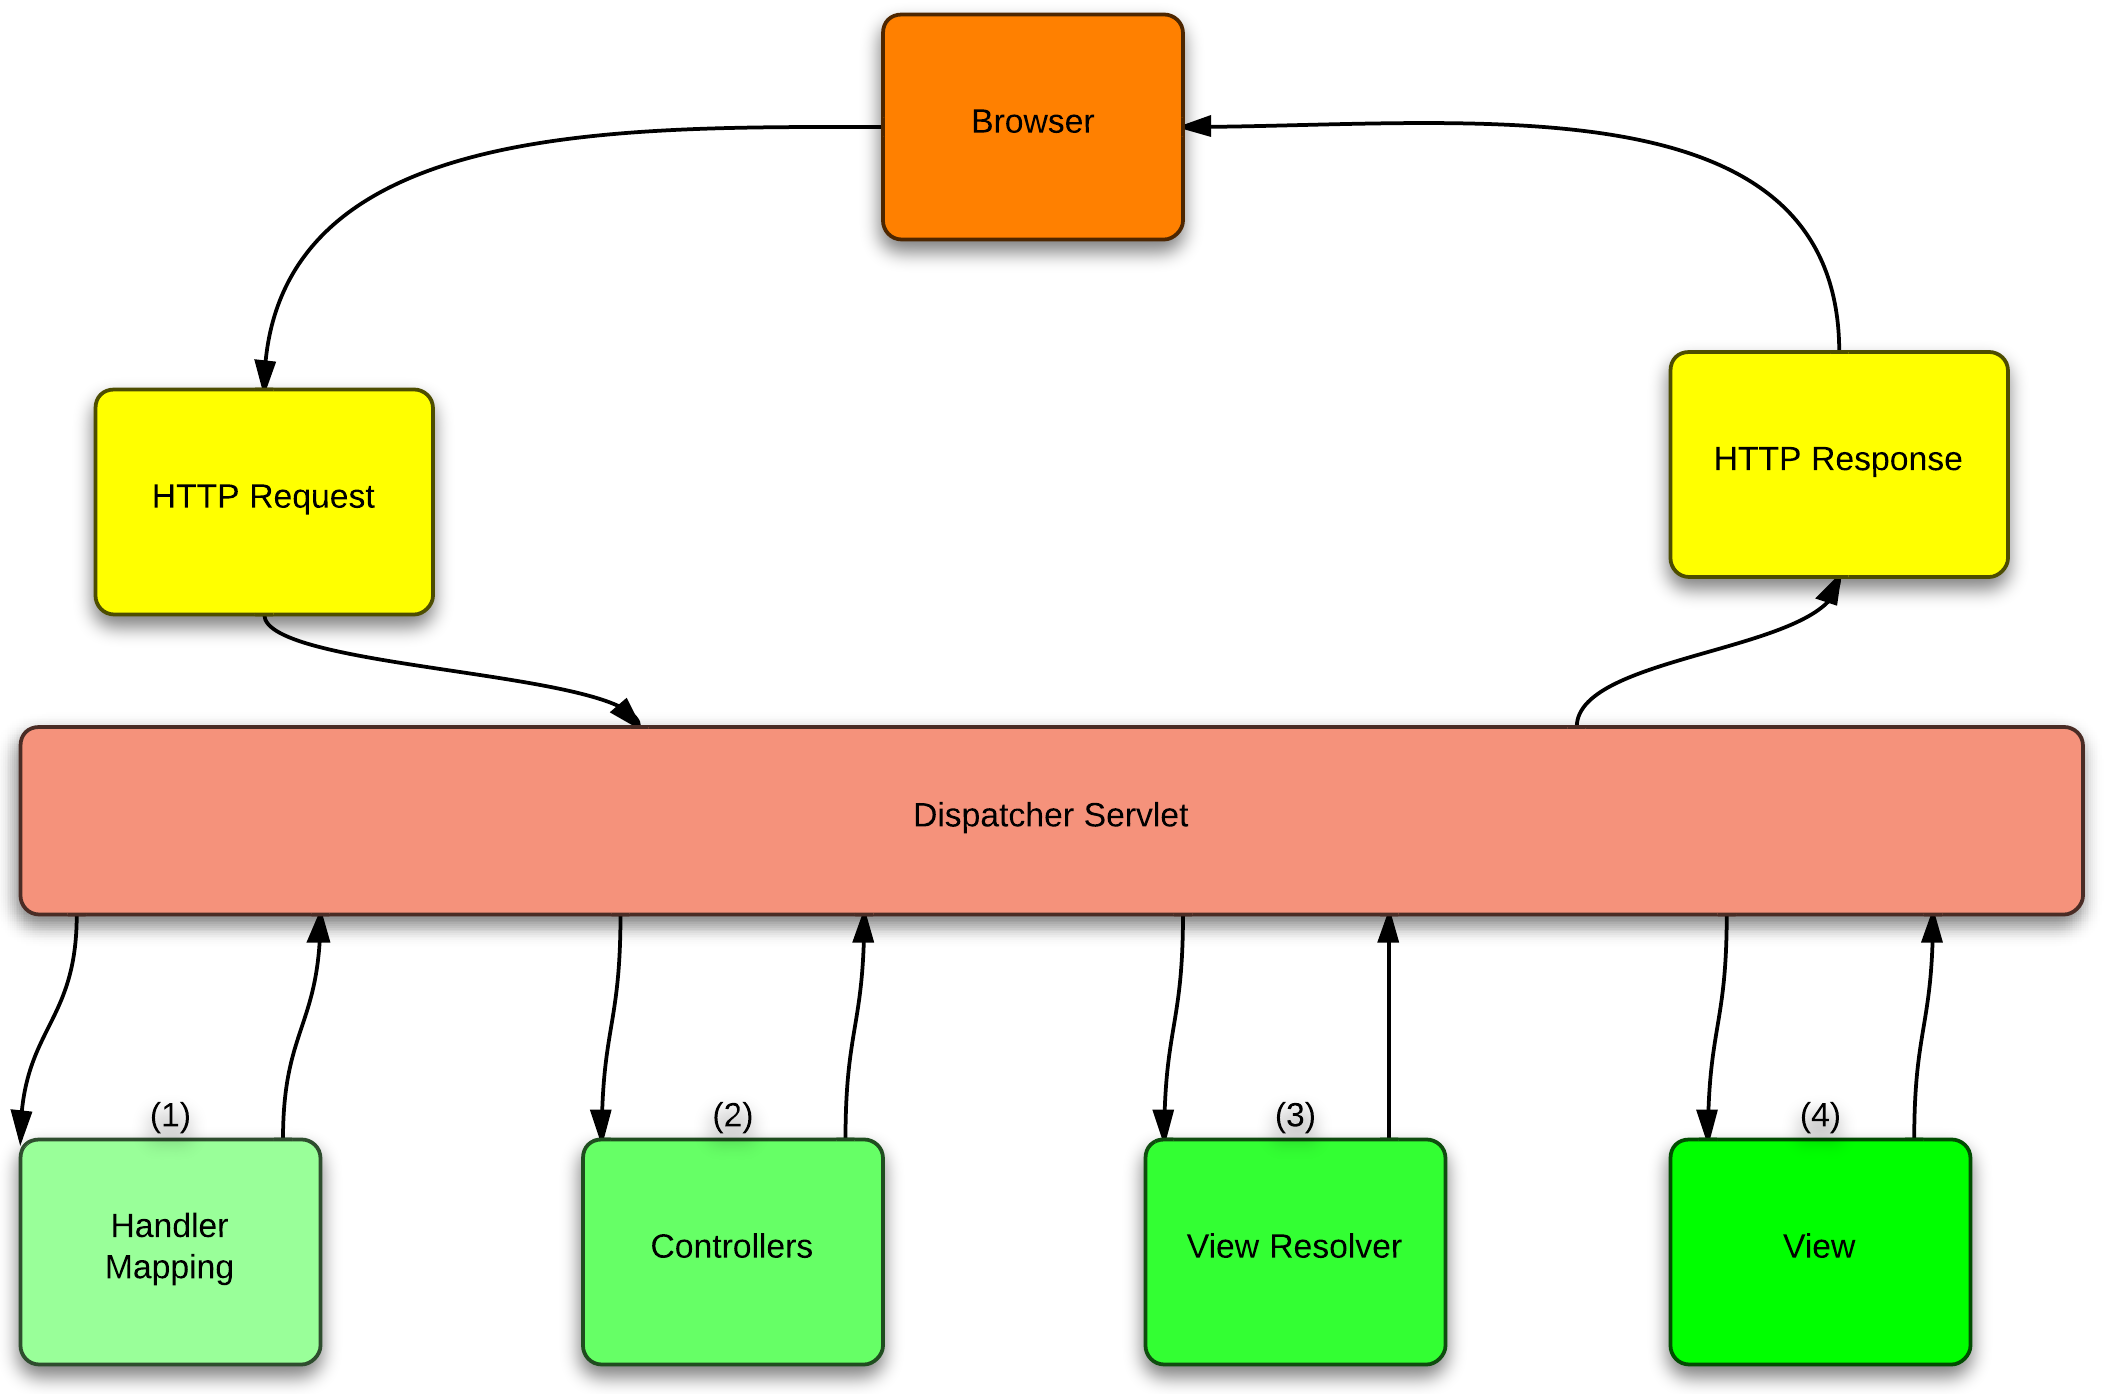
\includegraphics[width=9cm]{dispatchservlet.png}
\end{center}
\caption{DispatcherServlet }
\label{fig:dispatcherflow}
\end{table}

(NEEDS TO BE CITED!!!)


(Spring Core container handles DI)

\subsection{View Resolver}

\subsubsection{Structure}

\subsubsection{Language}

\subsection{Application Server}

\subsection{Project Management Tool}

\subsection{Database Model}

\subsection{Source Control}

\subsection{Integrated Development Environment}

\subsection{Logging}

\subsection{Version Control}




\section{Usability Studies}

\subsection{Case Study: Monaleen GAA Tennis Club}

\subsection{Case Study: Tralee Tennis Club}